\documentclass[a4paper,12pt]{article}
\usepackage{CJKutf8}
\usepackage{multirow}
\usepackage{graphicx}
\usepackage{amsmath}
\usepackage{amsfonts}
\usepackage{enumerate}
\usepackage{fancyhdr}
\usepackage{setspace}
\usepackage{bm}
%\pagestyle{fancy}
%\lhead{}
%\rhead{\bfseries Integral on lines and surfaces}
%\lfoot{Calculus}
%\cfoot{China University of Petroleum-Beijing}
%\rfoot{\thepage}
%\renewcommand{\headrulewidth}{0.4pt}
%\renewcommand{\footrulewidth}{0.4pt}
%%%% 段落首行缩进两个字 %%%%
\makeatletter
\let\@afterindentfalse\@afterindenttrue
\@afterindenttrue
\makeatother
\setlength{\parindent}{2em}  %中文缩进两个汉字位

\newcounter{solution}
\newcommand\TheSolution{%
  \textbf{Solution:}\\%
}

%%%% 下面的命令重定义页面边距,使其符合中文刊物习惯 %%%%
\addtolength{\topmargin}{-54pt}
\setlength{\oddsidemargin}{0.63cm}  % 3.17cm - 1 inch
\setlength{\evensidemargin}{\oddsidemargin}
\setlength{\textwidth}{14.66cm}
\setlength{\textheight}{24.00cm}    % 24.62

%%%% 下面的命令设置行间距与段落间距 %%%%
\linespread{1.4}
% \setlength{\parskip}{1ex}
\setlength{\parskip}{0.5\baselineskip}

%%%% 定理类环境的定义 %%%%
\newtheorem{example}{Example}             % 整体编号
\newtheorem{algorithm}{算法}
\newtheorem{theorem}{Theorem}[section]  % 按 section 编号
\newtheorem{definition}{Definition}
\newtheorem{axiom}{公理}
\newtheorem{property}{性质}
\newtheorem{proposition}{命题}
\newtheorem{lemma}{引理}
\newtheorem{corollary}{推论}
\newtheorem{remark}{注解}
\newtheorem{condition}{条件}
\newtheorem{conclusion}{结论}
\newtheorem{assumption}{假设}

%%%% 重定义 %%%%
\renewcommand{\contentsname}{目录}  % 将Contents改为目录
\renewcommand{\abstractname}{摘要}  % 将Abstract改为摘要
\renewcommand{\refname}{参考文献}   % 将References改为参考文献
\renewcommand{\indexname}{索引}
%\renewcommand{\figurename}{图}
\renewcommand{\tablename}{表}
\renewcommand{\appendixname}{附录}
\renewcommand{\algorithm}{算法}

\begin{document}
\begin{CJK}{UTF8}{gbsn}
\title{Elements of Vector Analysis and Field Theory}
\author{Guoning Wu\footnote{Email: wuguoning@163.com}\\[2ex]
 China University of Petroleum-Beijing\\[2ex]}
\date{2017.9}
\maketitle

\section{Maxwell's Equations}
Maxwell's equations are a set of partial differential equations that, 
together with the Lorentz force law, form the foundation of classical 
electromagnetism, quantum field theory, classical optics, and electric 
circuits. They underpin all electric, optical and radio technologies, 
including power generation, electric motors, wireless communication, 
cameras, televisions, computers etc. Maxwell's equations describe how 
electric and magnetic fields are generated by charges, currents, and 
changes of each other. One important consequence of the equations is 
that they demonstrate how fluctuating electric and magnetic fields 
propagate at the speed of light. Known as electromagnetic radiation, 
these waves may occur at various wavelengths to produce a spectrum 
from radio waves to $\gamma$-rays. The equations are named after the 
physicist and mathematician James Clerk Maxwell, who between 1861 and 
1862 published an early form of the equations, and first proposed 
that light is an electromagnetic phenomenon.

The equations have two major variants. The microscopic Maxwell equations 
have universal applicability, but are unwieldy for common calculations. 
They relate the electric and magnetic fields to total charge and total 
current, including the complicated charges and currents in materials 
at the atomic scale. The "macroscopic" Maxwell equations define two 
new auxiliary fields that describe the large-scale behaviour of matter 
without having to consider atomic scale details. However, their use 
requires experimentally determining parameters for a phenomenological 
description of the electromagnetic response of materials.

The term "Maxwell's equations" is often used for equivalent alternative 
formulations. Versions of Maxwell's equations based on the electric and 
magnetic potentials are preferred for explicitly solving the equations 
as a boundary value problem, analytical mechanics, or for use in quantum 
mechanics. The spacetime formulations (i.e., on spacetime rather than 
space and time separately), are commonly used in high energy and 
gravitational physics because they make the compatibility of the equations 
with special and general relativity manifest.[note 1] In fact, 
Einstein developed special and general relativity to accommodate 
the absolute speed of light that drops out of the Maxwell equations 
with the principle that only relative movement has physical consequences.

\section{Vector Operations in Curvilinear Coordinates}

    \paragraph{\textbf{a.}} Just as, for example, the sphere $x^2 + y^2 + z^2 = a^2$ has a 
    particularly simple equation $R = a$ in spherical coordinates,
    vector fields $x \to \bm{A}(x)$ in $\mathbb{R}^3$ (or $\mathbb{R}^n$)
    often assume a simpler expression in a coordinate system that 
    is not Cartesian. For that reason we now wish to find explicit 
    formulas from which one can find grad, curl and div in a rather 
    extensive class of curvilinear coordinates. But first it is 
    necessary to be precise as to what is meant by the coordinate 
    expression for a field $\bm{A}$ in a curvilinear system.

    We begin with two introductory examples of a descriptive 
    character.

    \begin{example}
        Suppose we have a fixed Cartesian coordinate system 
        $x^1, x^2$ in the Euclidean plane $\mathbb{R}^2$. When we say 
        that a vector field $(A^1, A^2)(x)$ is defined in $\mathbb{R}^2$,
        we mean that some vector $A(x) \in \bm{T}\mathbb{R}^2 $ is 
        connected with each point $x = (x^1, x^2) \in R^2$, and in the 
        basis of $\bm{T}\mathbb{R}^2$ consisting of the unit vectors 
        $\bm{e}_1(x), \bm{e}_2(x)$ in the coordinate directions we have 
        the expansion $\bm{A}(x) = A^1(x)\bm{e}_1(x) + A^2(x)\bm{e}_2(x)$
        (see Figure~\ref{fig:fig1}).In this case the basis 
        $\left\{ \bm{e}_1(x), \bm{e}_2(x)\right\}$ of $\bm{T}\mathbb{R}^2$
        is essentially independent of $x$.
    \end{example}
    \graphicspath{
        {./Figs/}
    }
    \begin{figure}[htbp]
    \centering
    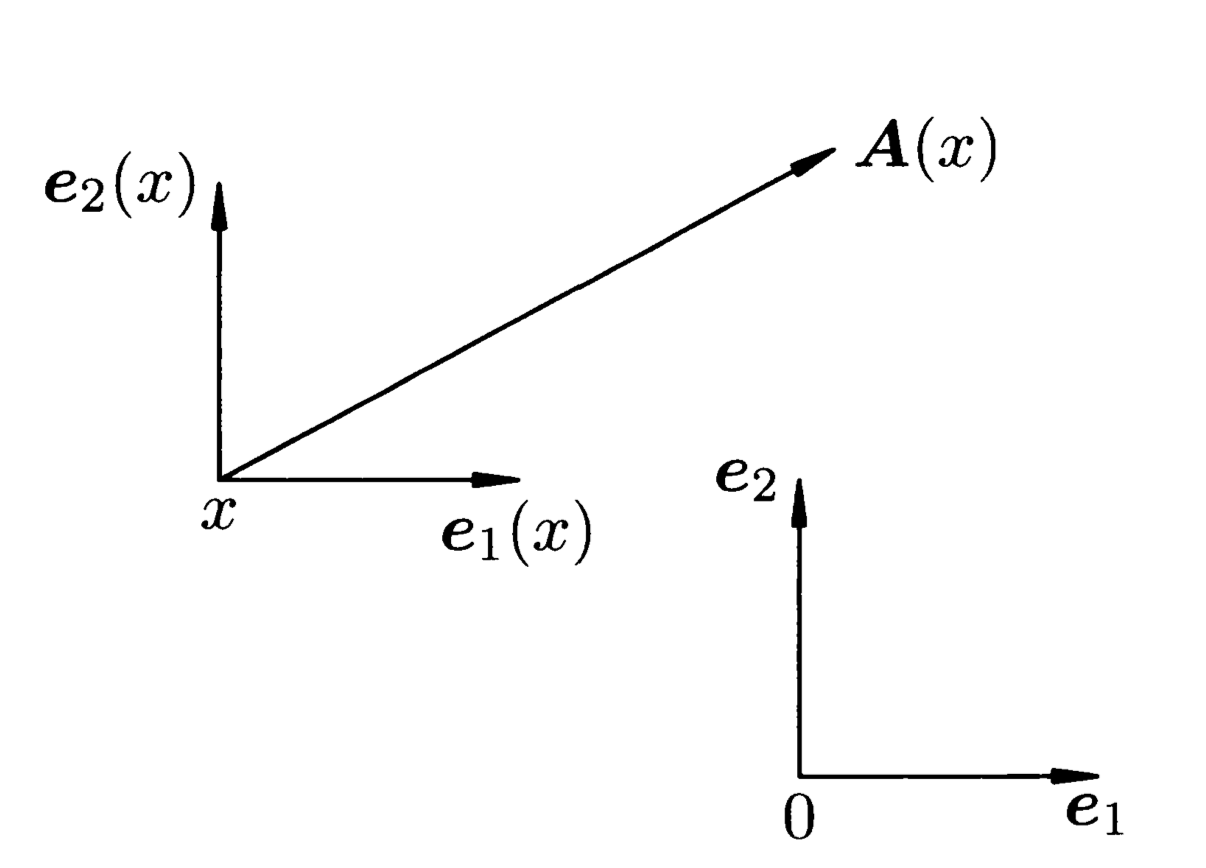
\includegraphics[width=0.5\textwidth]{vector_base1.png}
    \caption{Cartesian Coordinate.}
    \label{fig:fig1}
    \end{figure}

\begin{example}
    In the case when polar coordinate $\left(r, \varphi\right)$ are defined 
    in the same plane $\mathbb{R}^2$, at each point $x \in \mathbb{R}^2 
    \setminus 0$  one can also attach unit vectors $\bm{e}_1(x) = \bm{e}_r(x),
    \bm{e}_2(x) = \bm{e}_{\varphi}(x)$ (see Figure~\ref{fig:fig2})
    in the coordinate directions. They also form a basis in 
    $\bm{T}\mathbb{R}^2$ with respect to which one can expand the 
    vector $\bm{A}(x)$ of the field $\bm{A}$ attached to $x: 
    \bm{A}(x) = A^1(x)\bm{e}_1(x) + A^2(x)\bm{e}_2(x)$. It is then 
    natural to regard the ordered pair of functions $(A^1, A^2)(x)$
    as the expression for the field $\bm{A}$ in polar coordinate.

    Thus, if $(A^1, A^2)(x) \equiv (1, 0)$, this is a field of unit vectors 
    in $\mathbb{R}^2$ pointing radially away from the center 0.
    The field $\left(A^1, A^2\right)(x) \equiv \left(0,1\right)$ can be obtained from 
    the preceding field by rotating each vector in it counterclockwise 
    by the angle $\pi/2$.
\end{example}

These are not constant fields in $\mathbb{R}^2$, although the components 
of their coordinate representation are constant. The point is that 
the basis in which the expression is taken varies synchronously 
with the vector of the field in a transition from one point to another.
It is clear that the components of the coordinate representation of 
these field in Cartesian coordinates would not be constant at all.

\begin{figure}[htbp]
    \centering
    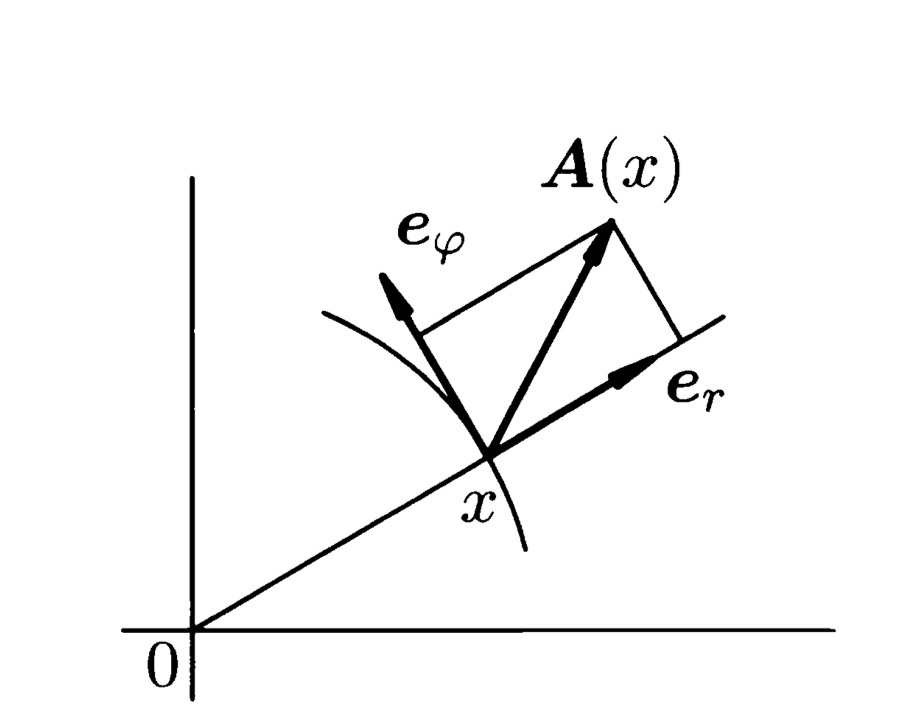
\includegraphics[width=0.5\textwidth]{vector_base2.png}
    \caption{Polar Coordinate.}
    \label{fig:fig2}
\end{figure}

\paragraph{\textbf{b.}} After these introductory consideration, let us
consider more formally the problem of defining vector fields in 
curvilinear coordinate systems.

We recall first of all that a curvilinear coordinate system $t^1, t^2, 
t^3$ in a domain $D \subset \mathbb{R}^2$ is a diffeomorphism $\varphi : 
D_t \to D$ of a domain $D_t$ in the Euclidean parameter space $\mathbb{R}^3$
onto the domain $D$, as a result of which each point $x = \varphi(t) \in D_t$
requires the Cartesian coordinates $t^1, t^2, t^3$ of the corresponding 
point $t \in D_t$.

Since $\varphi$ is a diffeomorphism, the tangent mapping $\varphi'(t): \bm{T}\mathbb{R}_t^3 
\to \bm{T}\mathbb{R}_x^3$ is a vector-space isomorphism. To the canonical basis 
$\xi_1(t) = \left(1, 0, 0\right), \xi_2(t) = \left(0, 1, 0\right), \xi_3\left(0, 0, 1\right)$
of $\bm{T}\mathbb{R}_t^3$ corresponds the basis of $\bm{T}\mathbb{R}_{x=\varphi(t)}^3$
consisting of the vectors $\xi_i(x) = \varphi'(t)\xi_i(t) = \frac{\partial \varphi(t)}{\partial t^i},
i=1,2,3$, giving the coordinate directions. To the expansion $\bm{A}(x)
= \alpha_1\xi_1(x) + \alpha_2\xi_2(x) + \alpha_3\xi_3(x)$ of any vector $\bm{A}(x) \in 
\bm{T}\mathbb{R}_x^3$ in this basis there corresponds the same expression 
$\bm{A}(t) = \alpha_1\xi_1(t) + \alpha_2\xi_2(t) + \alpha_3\xi_3(t)$ (with the same components 
$\alpha_1, \alpha_2, \alpha_3$) of the vector $\bm{A}(t) = \varphi^{-1}\bm{A}(x)$ in the 
canonical basis $\xi_1(t), \xi_2(t), \xi_3(t)$ in $\bm{T}\mathbb{R}_t^3$ .
In the absence of a Euclidean structure in $\mathbb{R}^3$, the number 
$\alpha_1, \alpha_2, \alpha_3$ would be the most natural coordinate expression 
for the vector $\bm{A}(x)$ connected with this curvilinear coordinate system.

\paragraph{\textbf{c.}} However, adopting such a coordinate representation 
would not be quite consistent with what we agreed to in Example above. 
The point is that the basis $\xi_1(x), \xi_2(x), \xi_3(x)$ in $\bm{T}\mathbb{R}_x^3$
corresponding to the canonical basis $\xi_1(t), \xi_2(t), \xi_3(t)$ in $\bm{T}\mathbb{R}_t^3$,
although it is consists of vectors in the coordinate directions, is not 
at all required to consist of \textit{unit vector} in those directions, that is,
in general $\langle \xi_i, \xi_i\rangle (t) \ne 1.$

We shall now take account of this circumstance which results from the 
presence of a Euclidean structure in $\mathbb{R}^3$ and consequently in 
each vector space $\bm{T}\mathbb{R}_x^3$ also.

Because of the isomorphism $\varphi'(t): \bm{T}\mathbb{R}_t^3 \to \bm{T}
\mathbb{R}_{x=\varphi(t)}^3$ we can transfer the  Euclidean structure 
of $\bm{T}\mathbb{R}_x^3$ into $\bm{T}\mathbb{R}_t^3$ by setting 
$\langle \tau_1, \tau_2 \rangle := \langle \varphi'\tau_1, \varphi'\tau_2 \rangle$
for every pair vector $\tau_1\, \tau_2 \in \bm{T}\mathbb{R}_t^3$. In particular, 
we obtain from this the following expression for the square of the 
length of a vector:
\begin{equation}
    \begin{split}
        \langle \tau, \tau \rangle & = \langle \varphi'(t)\tau, \varphi'(t)\tau \rangle
        \langle \frac{\partial \varphi}{\partial t^i}\tau^i, \frac{\partial \varphi}{\partial t^j}
        \tau \rangle \\
        & = \langle \frac{\partial \varphi}{\partial t^i}, \frac{\partial \varphi}{\partial t^j}
        \rangle (t)\tau^i\tau^j = \langle \xi_i, \xi_j\rangle (t)\tau^i\tau^j \\
        & = g_{ij}(t)\tau^i\tau^j = ds^2.
    \end{split}
\end{equation}

The quadratic form 
\begin{equation}
    \mathrm{d}s^2 = g_{ij}\mathrm{d}t^i\mathrm{d}t^j
\end{equation}
whose coefficients are the pairwise inner products of the vectors in the 
canonical basis determines the inner product on $\bm{T}\mathbb{R}_t^3$ 
completely. If such a form is defined at each point of a domain $D_t \subset 
\mathbb{R}_t^3$, then, as is known from geometry, one say that a 
\textit{Riemannian metric} is defined in this domain. A Riemannian metric makes 
it possible to introduce a Euclidean structure in each tangent space 
$\bm{T}\mathbb{R}_t^3 (t\in D_t)$ within the context of rectilinear coordinate 
$t^1, t^2, t^3$ in $\mathbb{R}_t^3$, corresponding to the curved embedding 
$\varphi: D_t \to D$ of the domain $D_t$ in the Euclidean space $\mathbb{R}^3$.
\end{CJK}
\end{document}
